\documentclass[12pt]{article}
\usepackage[margin=1in]{geometry} 
\usepackage{amsmath,amsthm,amssymb,amsfonts}
\usepackage[spanish]{babel}
\usepackage[utf8]{inputenc}
\usepackage{mathtools}
\selectlanguage{spanish}
\newcommand{\N}{\mathbb{N}}
\newcommand{\Z}{\mathbb{Z}}
\usepackage{color}
\usepackage{graphicx}
\usepackage[noend]{algorithmic}
\usepackage{comment}
\usepackage{float}
\usepackage{hyperref}
\newenvironment{solution}
  {\renewcommand\qedsymbol{$\blacksquare$}\begin{proof}[Solución]}
  {\end{proof}}

%pseudocodigo
\newcommand{\TITLE}[1]{\item[#1]}
\renewcommand{\algorithmiccomment}[1]{$/\!/$ \parbox[t]{4.5cm}{\raggedright #1}}
% ugly hack for for/while
\newbox\fixbox
\renewcommand{\algorithmicdo}{\setbox\fixbox\hbox{\ {} }\hskip-\wd\fixbox}
% end of hack
%imitando para if
\renewcommand{\algorithmicthen}{\setbox\fixbox\hbox{\ {} }\hskip-\wd\fixbox}
\newcommand{\algcost}[2]{\strut\hfill\makebox[1.5cm][l]{#1}\makebox[4cm][l]{#2}}

%piso techo 
\DeclarePairedDelimiter\ceil{\lceil}{\rceil}
\DeclarePairedDelimiter\floor{\lfloor}{\rfloor}
 
 \newenvironment{ejercicio}[2][Ejercicio]{\begin{trivlist}
\item[\hskip \labelsep {\bfseries #1}\hskip \labelsep {\bfseries #2.}]}{\end{trivlist}}

\newenvironment{problem}[2][Problem]{\begin{trivlist}
\item[\hskip \labelsep {\bfseries #1}\hskip \labelsep {\bfseries #2.}]}{\end{trivlist}}
%If you want to title your bold things something different just make another thing exactly like this but replace "problem" with the name of the thing you want, like theorem or lemma or whatever
 
\begin{document} 
%\renewcommand{\qedsymbol}{\filledbox}
%Good resources for looking up how to do stuff:
%Binary operators: http://www.access2science.com/latex/Binary.html
%General help: http://en.wikibooks.org/wiki/LaTeX/Mathematics
%Or just google stuff


 
\title{Proyecto Parcial\\
Analisis y Diseño de Algoritmos\\
\textsc{Universidad de Ingenieria y Tecnologia}
}
\author{Luis Ponce, Dario Toribio, Jonathan Hoyos}


\maketitle

\doublespacing
\tableofcontents
\singlespacing

\newpage

\section{Implementacion del Codigo}

El codigo se implemento en C++ y cuenta de 6 archivos.

\begin{itemize}
		\item \textbf{main.cpp} $\Rightarrow$ Inicio del programa
		\item \textbf{programa.h} $\Rightarrow$ Contiene la clase Programa. Encargada de recibir los inputs y parsearlos para luego guardarlos en un atributo de tipo Secuencia.
		\item \textbf{secuencia.h} $\Rightarrow$ Contiene la clase Secuencias. Encargada de almacenar los vectores con pesos y ejecutar el algoritmo voraz, recursivo y memorizado.
		\item \textbf{Makefile} $\Rightarrow$ Makefile para correr el proyecto.
		\item \textbf{run.sh} $\Rightarrow$ Script que corre el Makefile y corre el ejecutable obtenido.
		\item \textbf{parser.py} $\Rightarrow$ Codigo util para generar la tabla de resultados
		\item \textbf{tests} $\Rightarrow$ Una lista de 50 tests que el programa correra.
		\item \textbf{resultados}  $\Rightarrow$ Resultados de la ejecucion Voraz, recursiva y memoizada. Ademas cuenta los tiempos en ms de demora. 
		
\end{itemize}


\subsection{Variables importantes}
Lista de variables que seran utiles en el desarrollo del proyecto.\\

\begin{itemize}
		\item \textbf{A\_vector} $\Rightarrow$ Almacena el input original del primero arreglo. \textit{Ejm: \{1,1,0,1,0,1,1,0,0,1\}}
		\item \textbf{B\_vector} $\Rightarrow$ Almacena el input original del segundo arreglo. \textit{Ejm: \{1,1,0,1,1,0,0,0,1,1\}}
		\item \textbf{A\_weights} $\Rightarrow$ Almacena los pesos (cantidad de 1's juntos) del primer arreglo. \textit{Ejm: \{2,1,2,1\}}
		\item \textbf{B\_weights} $\Rightarrow$ Almacena los pesos (cantidad de 1's juntos) del segundo arreglo. \textit{Ejm: \{2,2,2\}}
		\item \textbf{A\_acumulado} $\Rightarrow$ Almacena los pesos acumulados del primero arreglo. Servira para no realizar calculos innecesarios en las funciones \textit{OPT(i,j)}. \textit{Ejm :\{2,3,5,6\}}
		\item \textbf{B\_acumulado} $\Rightarrow$ Almacena los pesos acumulados del segundo arreglo. Servira para no realizar calculos innecesarios en las funciones \textit{OPT(i,j)}. \textit{Ejm :\{2,4,6\}}
\end{itemize}



\newpage



\section{Solucion Voraz}

\subsection{Pseudocodigo}

\textbf{Recibe}: A\_weights, B\_weights

\textbf{Devuelve}: Suma de Agrupaciones y Divisiones. \\
\begin{algorithmic}[1]
		\TITLE{\textsc{Voraz\_func}$(A\_weights,B\_weights)$}
	
  \RETURN \textsc{voraz}$(A\_weights.size(),B\_weights.size())$
  
  \end{algorithmic}

\par\null\par

\begin{algorithmic}[1]
		\TITLE{\textsc{voraz}$(i,j)$}
  \IF{$i$ == 1 and $j$!=1}
  \RETURN A\_weights[$i$]/Sum\{B\_weights[$j:B\_weights.size()$]\}
  \ENDIF
  \IF{$j$ == 1 and $i$!=1}
  \RETURN Sum\{A\_weights[$i:A\_weights.size()$]\}/B\_weights[$j$]
  \ENDIF
  \IF{$i$ == 1 and $j$ == 1}  
  \RETURN A\_weights[$i$]/B\_weights[$j$]
  \ENDIF
  \STATE Auxiliar = B\_weights[$j$]
  \IF{A\_weights[$i$]/B\_weights[$j$] $> 1$}
  \WHILE{A\_weights[$i$]/B\_weights[$j$] $ > 1$}
  \STATE $j+=1$
  \IF{$j == B\_weights.size()$}
  \STATE $j-=1$
  \BREAK
  \ENDIF
  \STATE Auxiliar += B\_weights[j]
  \ENDWHILE
  \RETURN A\_weights[$i$]/B\_weights[$j$] + voraz($i+1$,$j+1$)

 \end{algorithmic}
 \subsection{Justificacion Voraz}
 Este algoritmo no siempre devolvera el valor mas optimo, esto debido a que el ultimo match siemrpe es el peor, y siempre podrán haber mejores matches finales. Estamos encontrando minimos locales. La forma de encontrar los verdaderos minimos es aplicando un algoritmo Recursivo, Memoizado o Dinamico.

 \subsection{Complejidad de tiempo}

 El algoritmo Voraz realiza una recursion aumentando los $i,j$ en $1$ n caso la division del $A\_weights[i]/B\_weights[j] \leq 1$.\\
 En caso no sea menor se dividira $A\_weights[i]$ entre la suma de los $B\_weights[j \dots k]$ hasta que sea menor o igual a 1.\\
 Finalmente si llega al extremo del minimo, ejecutara un $FOR$ para encontrar su suma de pesos hasta el final, $Arr\_max[pos\_actual : pos\_final]$ y realizar la division o agrupacion, dependiendo cual es el vector con mayor tamaño.\\ \\
 De esta manera queda demostrado que el algoritmo tiene complejidad de tiempo $O(Max\{A,B\})$


\newpage
\section{Solucion Recursiva}

\subsection{Pseudocodigo}

\textbf{Recibe}: A\_weights, B\_weights

\textbf{Devuelve}: Minima Suma de Agrupaciones y Divisiones. \\
\begin{algorithmic}[1]
		\TITLE{\textsc{Recursivo\_func}$(A\_weights,B\_weights)$}
	
  \RETURN \textsc{opt}$(A\_weights.size(),B\_weights.size())$
  
  \end{algorithmic}

\par\null\par

\begin{algorithmic}[1]
		\TITLE{\textsc{OPT}$(i,j)$}
  \IF{$i$ == 1 and $j$!=1}
  \RETURN A\_weights[$i$]/B\_acumulado[$j$]
  \ENDIF
  \IF{$j$ == 1 and $i$!=1}
  \RETURN A\_acumulado[$i$]/B\_weights[$j$]
  \ENDIF
  \IF{$i$ == 1 and $j$ == 1}  
  \RETURN A\_weights[$i$]/B\_weights[$j$]
  \ENDIF
  \STATE $Valores[:]$
  \FOR{$k=j$ \TO 2} 
  \STATE
  $\begin{aligned}
  Valores \Leftarrow (A\_weights[$i$]/(B\_acumulado[$j$] - B\_acumulado[$k-1$]) + OPT($i-1$,$k-1$))
  \end{aligned}$
  \ENDFOR
  \FOR{$k=i$ \TO 2}
  \STATE 
  $\begin{aligned}
  $Valores$ \Leftarrow ((A\_acumulado[$i$] - A\_acumulado[$k-1$])/B\_weights[$j$] + OPT($k-1$,$j-1$))
  \end{aligned}$
  \ENDFOR
 
  \RETURN $minimo (Valores)$

\end{algorithmic}

\subsubsection{Explicacion del pseudocodigo}

Funcionamiento de los dos \textit{for} en las lineas $8-11$ en el pseudocodigo \textbf{OPT}

 \begin{figure}[h]
		 \centering
		 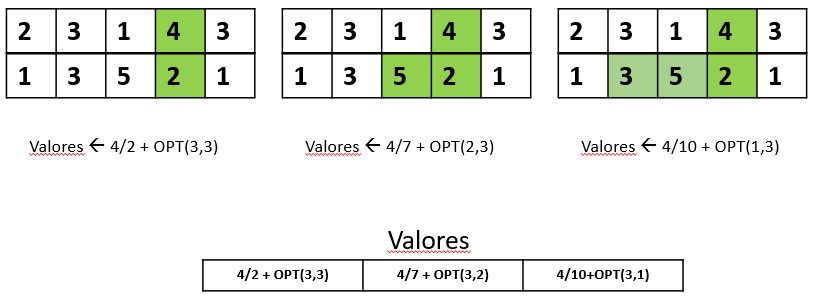
\includegraphics[width=40em, height=12em]{ejemplo2.PNG}
		 \caption{Datos guardados por Valores en el primer for}
 \end{figure}

 
 \begin{figure}[h]
		 \centering
		 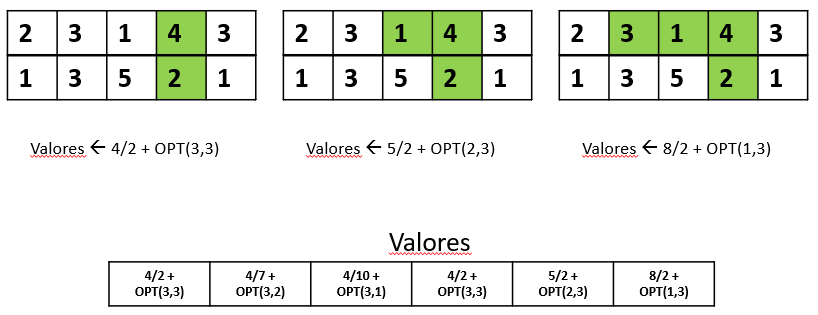
\includegraphics[width=40em, height=12em]{ejemplo3.PNG}
		 \caption{Datos guardados por Valores en el segundo for}
 \end{figure}

 El fin es calcular todos los posibles casos que se podrian encontrar si utilizamos esos \textit{i,j}. Luego de calcular dichos valores se retorna el minimo de este vector, el cual contiene la minima suma al usar agrupamientos y divisiones en esos indices.


\subsection{Recursion}
 \begin{itemize}
		 \item A\_w $\Rightarrow$ A\_weights
		 \item A\_acu $\Rightarrow$ A\_acumulado
		 \item B\_w $\Rightarrow$ B\_weights
		 \item B\_acu $\Rightarrow$ B\_acumulado
 \end{itemize}

\begin{equation*}
OPT(i,j) =
\begin{cases}
		A\_w[i]/B\_w[j] & \textbf{\text{i = 1 , j = 1}}\\
		A\_acu[i]/B\_w[j] & \textbf{\text{i!= 1, j = 1}}\\
		A\_w[i]/B\_acu[j] & \textbf{\text{i = 1 , j!= 1}}\\
\\
\textbf{Min\{ } &\\
		A\_w[i]/(B\_acu[j] - B\_acu[j-1]) + OPT(i-1,j-1), &\\
		A\_w[i]/(B\_acu[j] - B\_acu[j-2]) + OPT(i-1,j-2),  &\\
		\dots  \dots  &\\
		A\_w[i]/(B\_acu[j] - B\_acu[1]) + OPT(i-1,1), &\\
		& \textbf{\text{caso contrario}}\\
		(A\_acu[i] - A\_acu[i-1])/B\_w[j] + OPT(i-1,j-1), &\\
		(A\_acu[i] - A\_acu[i-2])/B\_w[j] + OPT(i-2,j-1), &\\
		\dots \dots &\\
		(A\_acu[i] - A\_acu[1])/B\_w[j] + OPT(1,j-1), &\\
\textbf{\}} \\
\end{cases}
\end{equation*}

Demostraremos por induccion que $OPT(n,m)\geq ck^{max(n,m)}$.\\ \\
Primero asumiremos a los tres casos no recursivos que son iguales a una variable $d$. Entonces: \\ \\
Para $k=\frac{3}{2}$ y $c\leq \frac{2d}{3}$.  \\ \\
Cuando ($i=1$ y $j=1$),($i=1$ y $j!=1$) o ($i!=1$ y $j=1$) y  tenemos que $OPT(i,j) = d \geq c$ 


\begin{eqnarray*}
		OPT(i,j)&=&q_1 + Min\{(OPT(i-1,j-1),OPT(i-2,j-1), \dots , OPT(1,j-1) \\
				&&OPT(i-1,j-1),OPT(i-1,j-2), \dots , OPT(i-1,1)\} \\
				OPT(i,j)&\geq&q_1 + Min\{ck^{Max(i-1,j-1)}, ck^{Max(i-2,j-1)}, \dots ,ck^{Max(1,j-1)},\\ 
				&&ck^{Max(i-1,j-1)}, ck^{Max(i-1,j-2)}, \dots , ck^{Max(i-1,1)}\}

\end{eqnarray*}

Debido a la funcion recursiva, se tienen que realizar dichos calculos de $OPT()$:

\begin{eqnarray*}
		&=&q_1 + ck^{Max(i-1,j-1)}+ck^{Max(i-1,j-2)}+ \dots + ck^{Max(i-1,1)} \dots \\
		&=&q_1 + ck^{Max(i,j)}(\frac{1}{k} + \frac{1}{k^2} + \dots + \frac{1}{k^{Max(i,j)-Min(i,j)}}+ \frac{1}{k^{Max(i,j)-Min(i,j)}}+ \dots + \frac{1}{k} + \frac{1}{k} + \dots + \frac{1}{k})

\end{eqnarray*}

Reemplazamos $k$ con $\frac{3}{2}$ y nos damos cuenta que: 

\begin{eqnarray*}
		OPT(i,j)&\geq&q_1+ck^{Max(i,j)}*1\\
\end{eqnarray*}

Por lo tanto, el tiempo de ejecucion del algoritmo recursivo es de $\Omega(2^{n})$
\newpage

\section{Solucion Memoizada}
\subsection{Pseudocódigo}
\textbf{Recibe}: A\_weights, B\_weights

\textbf{Devuelve}: Minima Suma de Agrupaciones y Divisiones.

\begin{algorithmic}[1]
		\TITLE{\textsc{Memoizado}$(i,j)$}
  \IF{$Matriz[i][j]$ != 0}
  \RETURN Matriz[i][j]
  \ENDIF
  \STATE $Valores[:]$
  \FOR{$k=j$ \TO 2} 
  \STATE
  $\begin{aligned}
  Valores \Leftarrow (A\_weights[$i$]/(B\_acumulado[$j$] - B\_acumulado[$k-1$]) + OPT($i-1$,$k-1$))
  \end{aligned}$
  \ENDFOR
  \FOR{$k=i$ \TO 2}
  \STATE 
  $\begin{aligned}
  $Valores$ \Leftarrow ((A\_acumulado[$i$] - A\_acumulado[$k-1$])/B\_weights[$j$] + OPT($k-1$,$j-1$))
  \end{aligned}$
  \ENDFOR
\STATE Matriz[i][j] = minimo(Valores)
  \RETURN $minimo (Valores)$
\end{algorithmic}

\par\null\par

\begin{algorithmic}[1]
        \TITLE{\textsc{CasoBase}$()$}
        \FOR{$i=1$ \TO A\_weights.size()}
        \STATE
        $\begin{aligned}
        Matriz[i][1] = A\_acumulado[$i$]/B\_weights[$1$]
        \end{aligned}$
        \ENDFOR
        \FOR{$i=1$ \TO B\_weights.size()}
        \STATE
        $\begin{aligned}
        Matriz[1][i] = A\_weights[$1$]/B\_acumulado[$i$]
        \end{aligned}$
        \ENDFOR
\end{algorithmic}

\par\null\par

\begin{algorithmic}[1]
        \TITLE{\textsc{Memoizado_func}$()$}
        \STATE CasoBase()
        \RETURN $Memoizado(A\_weights.size(), B\_weights.size())$
\end{algorithmic}
\subsubsection{Explicación del pseudocódigo}
La lógica aplicada en este algoritmo es la misma que en el algoritmo recursivo, solo que aquí guardamos los resultados que nos salgan para usarlos luego. \\
Primero, inicializamos el caso base, que viene siendo la primera fila y columna de la matriz, la cual al inicio esta llena de ceros. 
Una vez inicializado, aplicamos el algoritmo del recursivo, solo que aquí, antes de devolver el resultado, lo guardamos en su posición respectiva de la matriz. Por lo que, cada vez que se entre a la función recursivamente, se preguntara si esa posición 0, si es asi, continua el algoritmo, pero si este no es 0 significa que este valor ya fue calculado previamente. \\
\subsection{Complejidades}
Como podemos visualizar, el árbol recursivo tiene unos pocos niveles de más, esto es porque siempre opera todo lo que necesita, así ya lo haya calculado previamente. 
 \begin{figure}[H]
		 \centering
		 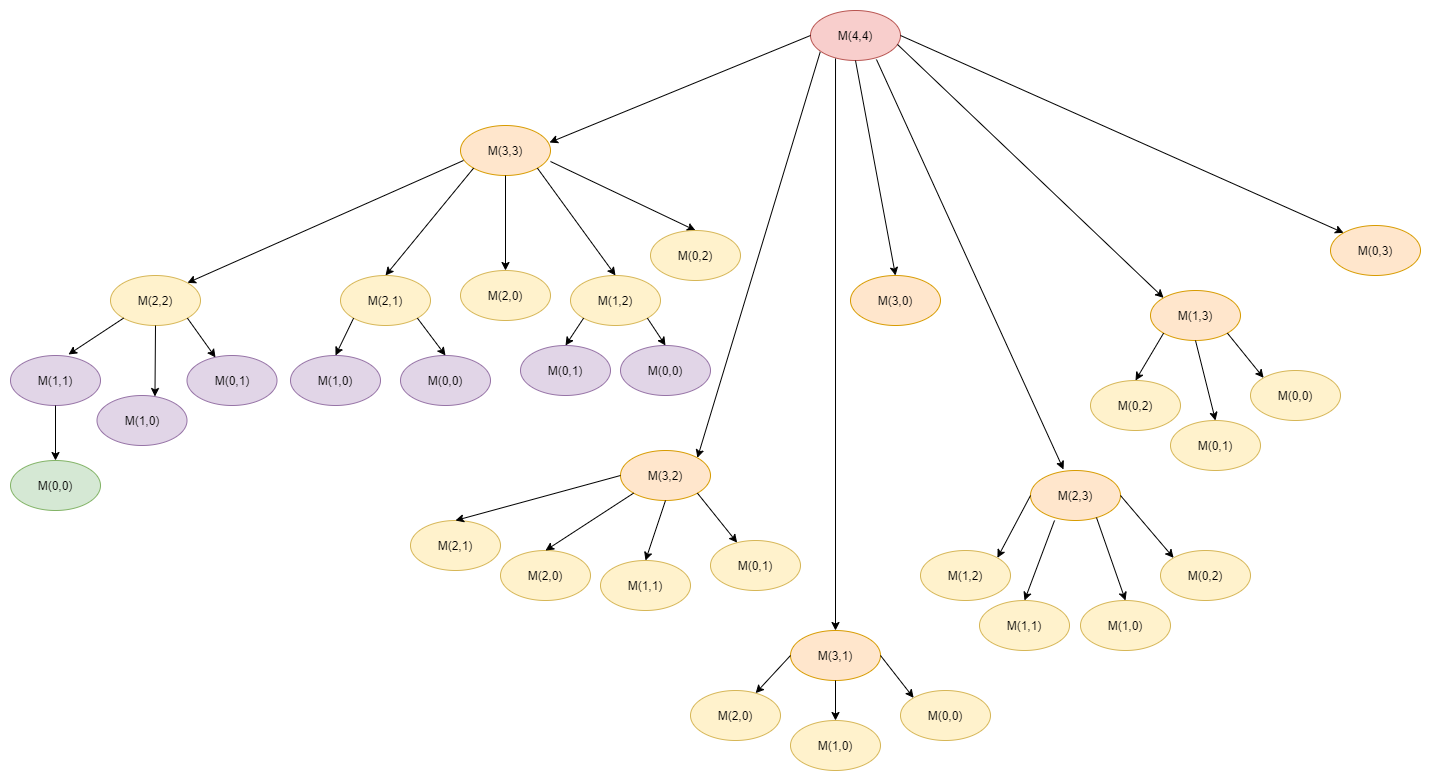
\includegraphics[width=33em, height=15em]{Memoizado_Arbol.png}
		 \caption{Árbol de recursión del algoritmo Memoizado para 2 arreglos de 4 valores}
 \end{figure}
  \begin{figure}[H]
		 \centering
		 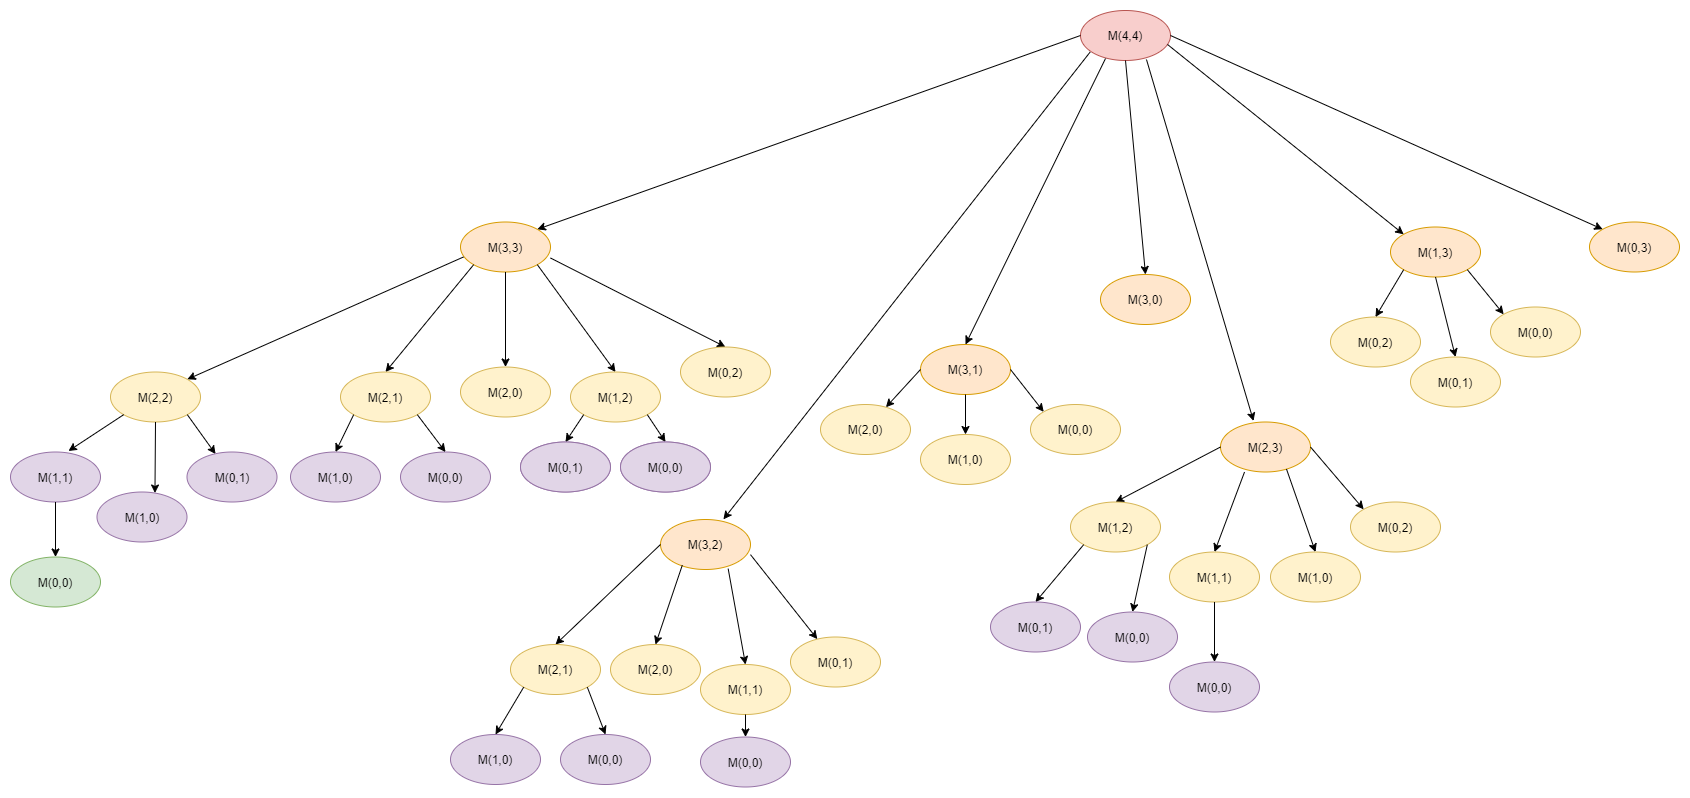
\includegraphics[width=33em, height=15em]{Recursivo arbol.png}
		 \caption{Árbol de recursión del algoritmo Memoizado para 2 arreglos de 4 valores}
 \end{figure}
\subsubsection{Complejidad Espacial}
Todos los valores se guardan en una matriz, teniendo siempre el valor óptimo para la submatriz i, j.
Por lo que al final el tamaño de esta matriz sería MxN.
\begin{figure}[H]
		 \centering
		 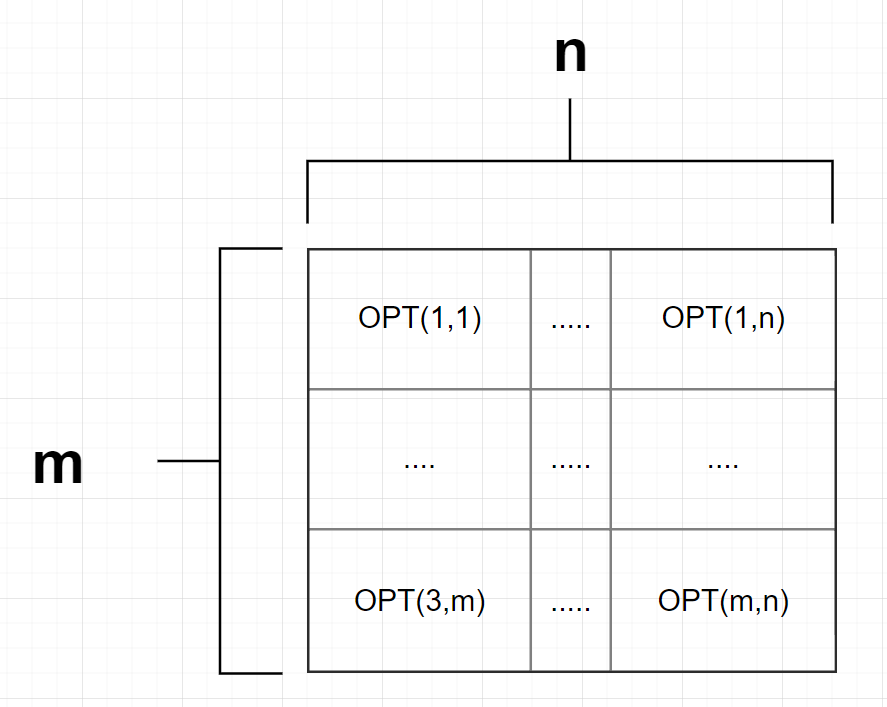
\includegraphics[width=20em, height=15em]{Matriz.png}
		 \caption{Complejidad de espacio}
\end{figure}
 
 
\subsubsection{Complejidad de tiempo}
Al inicio tienes la recursión T(m, n), el cuál comienza a generar los valores de la matriz en la primera recorrida, luego el resto de casillas se va llenando de acuerdo a lo que se necesita mas adelante. Esto hace que al calcular ciertas casillas, no tengamos que resolver OPT's anteriores porque estos a fueron guardados en la matriz. El máximo recorrido que hacemos sería desde el OPT(1,1) hasta el OPT(m,n), por lo que esta complejidad viene siendo dada por O(m*n)


\section{Github}
\href{https://github.com/LuchoPonceC/ADA-project}{Link del Proyecto}


\end{document}
